\section{Evaluation}
\label{sec-evaluation}

\begin{figure}[t]
%\begin{minipage}[b]{.45\linewidth}
    \includegraphics[width=.75\columnwidth, angle=270]{resultdata/onebigtimegraph.eps}
	\caption{Time for PolyPassHash operations.  The plots for thresholdless
creation and verification overlap as do the plots for the threshold versions
of each action.}
	\label{fig:time_basic_operations}  
\end{figure}
%\end{minipage}
%\hspace{.06\linewidth}
%\begin{minipage}[b]{.45\linewidth}
%    \includegraphics[width=.75\textwidth, angle=270]{resultdata/onebigperformancegraph.eps}
%	\caption{Performance (operations per second) for PolyPassHash operations.  }
%	\label{fig:performance_basic_operations}  
%\end{minipage}
%\end{figure*}
This section describes a performance evaluation of our prototype of 
PolyPassHash.   
To understand the performance of PolyPassHash,
we performed a series of microbenchmarks on an early-2011 MacBook Pro with 
4GB of RAM, a 2.3 GHz Intel Core i5 processor.  


%\begin{figure}[t]
%    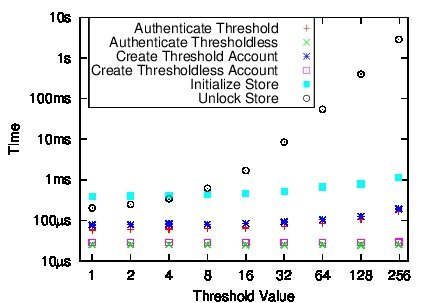
\includegraphics[width=0.3\textwidth,angle=270]{resultdata/onebigtimegraph}
%	\caption{Time for basic PolyPassHash operations.  }
%	\label{fig:time_basic_operations}  
%\end{figure}
%
%\begin{figure}[t]
%    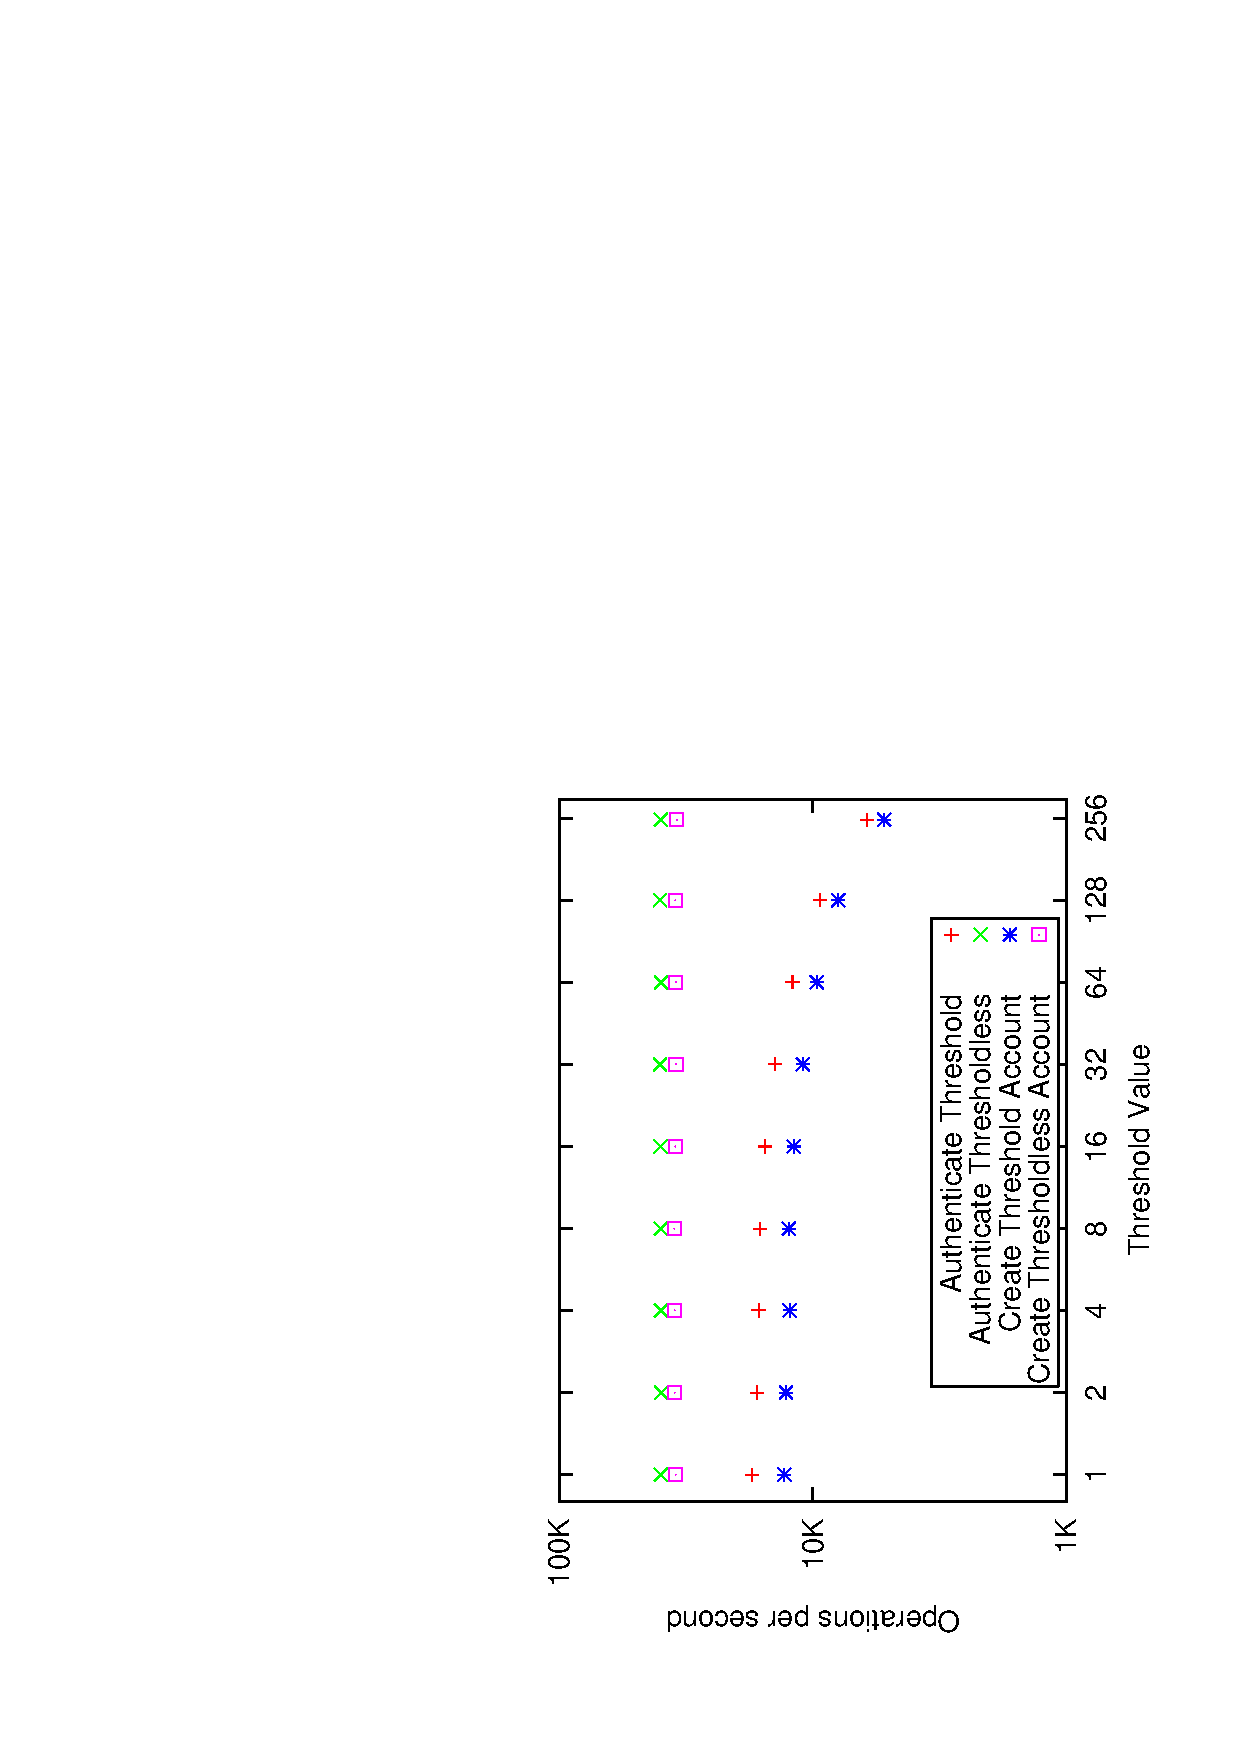
\includegraphics[width=0.3\textwidth,angle=270]{resultdata/onebigperformancegraph}
%	\caption{Performance (users impacted by an operation per second) for basic PolyPassHash operations.  }
%	\label{fig:performance_basic_operations}  
%\end{figure}

All operations are the mean verification time across 100 runs and
are performed with the password file already present in
memory.  
For benchmarking purposes, each action is performed sequentially despite being 
embarrassingly parallelizable.


\subsection{Performance Of A PolyPassHash Store}

%To evaluate the performance implications of PolyPassHash, we varied the 
%threshold.   While we do not believe that
%there will be many (if any) practical situations where the threshold would be 
%set to a value larger than ten.
%However, for completeness, we show the result of varying the threshold
%across a broader range of possible values.   
Figure~\ref{fig:time_basic_operations} shows the time taken by
different operations (discussed below).  Unless noted below,
the time of the operations does not depend on other factors such as the 
number of accounts in the password database.




{\bf Account Verification.}
The mean verification time of a threshold account
varies from 57$\mu$s to 163$\mu$s depending on the
threshold.  With a threshold of 8, this allows the verification of 
more than 16K user accounts per second.

Thresholdless accounts are verified in a time that is independent
of the threshold size because it merely computes    
a salted hash and performs an AES encryption operation.
Verifying
a thresholdless account takes about 29$\mu$s, allowing
about 35K such actions to be performed each second.   
In comparison, the current
best practice of generating the SHA256 hash of a known salt is a little over
3$\mu$s on the same hardware, which allows hundreds of thousands of
account authentications per second.   
%Note if there were a case where the account 
%validation software needed to process more than 35K account authorization
%attempts per second, the process is embarrassingly parallelizable.



{\bf Account Creation / Password Change.}
The account creation time is similar to that of password verification.
Depending on the threshold, the average verification time 
varies from 77$\mu$s to 190$\mu$s.  
A store with a threshold of 8 can create more than 12K 
accounts per second.   Given there are a maximum of 255 threshold accounts
that can be created (at least with a PolyPassHash implementation that uses
GF256), this clearly is not a performance concern.


Much like account verification, thresholdless accounts can be created in 
time that is independent of the threshold.   
A thresholdless account creation takes about 25$\mu$s.   As a result, 
about 40K thresholdless accounts can be created each second.   This is
similar to the time it takes to generate a salted SHA256 hash for a 
provided password (16$\mu$s). 

Note that changing the password requires that PolyPassHash performs the same
operation as account creation (potentially along 
with authentication of the old password).


{\bf Initializing a Store.}
The time to create a store varies depending on the threshold.   This
cost is dominated by generating cryptographically-suitable random
numbers.   By varying the threshold, the creation time varies from 
380$\mu$s to 1.13ms.   This operation is only performed when a 
new password file is created.

{\bf Unlocking a PolyPassHash Store.}
When the server restarts, the
random coefficients are computed from the set of provided shares with
full interpolation.   The time needed varies 
between 202$\mu$s and 2.87s as the threshold changes since
the number of polynomials changes as the store size grows.
Note that small thresholds are very fast, with a store with a threshold of 8
being unlocked in 617$\mu$s.

This is fast enough that if some passwords are incorrectly entered, 
PolyPassHash can (na\"ively) detect them.   For example, suppose that
a threshold of 10 is used and that 14 passwords are provided and only
10 of them are correct.   All possible combinations of 10 passwords can be
checked by PolyPassHash in 618ms.
Partial verification will also discard most passwords that are entered 
incorrectly to prevent them from being used to attempt to unlock the 
password store.
% If there is a huge threshold with a large number of
%candidate logins and passwords, it would also
%be possible to apply more advanced techniques for detecting incorrect
%shares~\cite{carpentieri1995perfect,Yang_compsac_02,devet2012optimally}.


%Furthermore, this process needs only to be performed when the 
%system is restarted.  


\subsection{Memory and Storage Costs of PolyPassHash}


\begin{table}[t]
{\scriptsize
\begin{tabular}{|l|l|l|l|}
\hline
Password & Original & Salted, Hashed & PolyPassHash \\
Source & Disk Space & Disk Space & Disk Space\\
\hline
\hline
eHarmony* & 51.6MB & 100MB & 102MB \\
\hline
Formspring* & 27.3MB & 34.8MB & 35.2MB \\
\hline
Gawker & 75.2MB & 119MB & 120MB \\
\hline
LinkedIn* & 252MB & 424MB & 430MB \\
\hline
Sony & 2.98MB & 4.95MB & 5.00MB  \\
\hline
Yahoo & 17.8MB & 35.0MB & 35.4MB \\
\hline
\end{tabular}
}
\caption{Disk space to store password data from different account disclosures.
Entries with a * indicate only the password hash portion of the database
was leaked.   Other breaches include usernames and similar data.  }
	\label{tab:extrahashcost}  
\end{table}



%\begin{table}[t]
%{\scriptsize
%\begin{tabular}{|l|l|l|}
%\hline
%Storage Mechanism & Disk per entry & Total memory cost\\
%\hline
%\hline
%Salted Secure Hash & 48 bytes & N/A (stored on disk) \\
%\hline
%Threshold & 49 bytes & $k*32$ bytes (likely $<1$KB) \\
%\hline
%Thresholdless (separate file) & 48 bytes & N/A (included in threshold) \\
%\hline
%Thresholdless (same file) & 49 bytes & N/A (included in threshold) \\
%\hline
%\end{tabular}
%}
%\caption{Cost to store the password hash database for PolyPassHash and 
%conventional salted hash techniques in terms of memory and disk space.
%A 16 byte salt and 32 byte hash is assumed for all schemes.}
%	\label{tab:extracost}  
%\end{table}

Storing passwords with PolyPassHash requires additional information be stored
for each account.   Namely, for each account, since each share is a value
in GF256, there must be a one byte share number stored for each account.   
This represents an additional 1 byte of storage space for each account in 
addition to the cost of current hash techniques.   This
has a minimal impact on the disk space needed to store production
password databases (Table~\ref{tab:extrahashcost}).   If the thresholdless 
accounts are stored in a separate file or are
otherwise distinguished, then only threshold accounts require the extra
byte of storage.   This will result in a cost for those accounts that is
identical to the salted, hashed scheme.

In addition, any account that has 
multiple entries (to count multiple times toward the threshold), requires an 
additional salt (16 bytes), hash (32 bytes), and share number (1 byte)
for every entry after the first.
Since there are at most 255 Shamir secret shares in GF256, this can be treated 
as a fixed cost of a few kilobytes.
%We do not believe the additional storage 
%cost will prove a burden in any practical scenario.

There is additional memory cost because the server must cache
the polynomial coefficients for a store.   The total
size of this data is the threshold value multiplied by the hash length.
Thus, the in-memory threshold data is likely to be under a 
kilobyte in practice.% (Table~\ref{tab:extracost}).   This is likely to be smaller than the (also minimal)
%memory space needed to store the additional code for PolyPassHash.
When thresholdless accounts are used, the AES key used is the 
constant term 
of the polynomial coefficients and so does not incur additional cost.
The use of partial verification has essentially no impact on the storage or 
memory requirements.

%Note that if thresholdless accounts are used and stored in the same
%file as threshold accounts, the disk costs
%are the same for both types of accounts (Table~\ref{tab:extracost}).   
%In order to indicate an account is thresholdless while using the same
%password database, the share number can be 
%set to 0 (an invalid share in traditional Shamir Secret Sharing).
%%There is the same memory and disk storage costs for each account regardless
%%of whether or not it counts toward the threshold.
%This indicates the account is thresholdless while permitting storage
%in the same file.




%\subsection{Thresholdless Accounts}
%
%\cappos{AES can compute about 400K 256 byte decryptions per second on my 
%laptop.   This is much faster than even SHA256, so should be much faster than
%accounts with a threshold.}


\subsection{Feasibility Of Cracking Passwords}
\label{sec-feasibility}

\begin{figure}[t]
\hspace{-4mm}
\includegraphics[width=.36\textwidth, angle=270]{resultdata/plotcrack.eps}
	\caption{Time to crack a password store given 1 billion attempts
per second.   The k=1 case for PolyPassHash is the same as the
legacy salted hash scheme.   The partial verification values show 
how leaking 2 bytes impacts cracking time.   A threshold of 3 without partial 
verification falls well outside the axis of the graph.}
	\label{fig:cracktime}  
\end{figure}

%Assuming a threshold of accounts is not known, cracking passwords takes 
%exponentially more time with PolyPassHash than standard hash
%schemes.   The reason is that an attacker must simultaneously attempt to
%crack the threshold number of passwords at once.
%An attacker must attempt to determine the random coefficients that are 
%protected by Shamir Secret Sharing before validating passwords.   This means 
%the attacker must know enough passwords to have at least the 
%threshold number of passwords.
%If an attacker needs to guess $p$ passwords, where each password has $V$ 
%possible values, the attacker is choosing values from $V^p$ possible guesses.   
%Solutions that involve slower hash functions or multiple hash iterations 
%result in only a linear increase in attack time and verification time.
%Since passwords must be correctly guessed simultaneously with PolyPassHash, 
%PolyPassHash results in an \emph{exponential} increase in attack time.

{\bf General Analysis.}
Even when an attacker needs to guess only a few passwords, in many cases 
PolyPassHash's \emph{exponential increase} in guessing time ($O(V^p)$ instead 
of $O(pV)$) makes guessing computationally infeasible 
(Figure~\ref{fig:cracktime}).   For example, suppose 
an attacker wants to guess three passwords that they know are each comprised 
of 6 randomly chosen characters\footnote{These passwords
are extremely weak and we do not advocate their use.   This 
example is used to illustrate the strength of PolyPassHash even with 
weak passwords.}.  Recent results 
have shown that a GPU can compute on the order of a billion password hashes a 
second~\cite{ElcomSoftGPUCracking, zonenberg2009distributed}, allowing the 
attacker to search the key space for all three passwords in under an hour.
Thus the current state of the art provides little protection in this case.

In the case of PolyPassHash, the attacker must \emph{simultaneously}
guess all three passwords.   This means the attacker needs to guess from 
$3.97 \times {10^{35}}$ values.   This is roughly 23 orders of magnitude more effort.
When PolyPassHash is used with the same passwords and the GPU 
accelerated technique, searching the key space would take $1.25 \times 10^{19}$
CPU years (does not fit on the axis of Figure~\ref{fig:cracktime}).   To put 
this number into context,
ignoring smartphones there are about 900 million computers on the 
planet~\cite{computersexisting}.   The estimated age of the universe is 
$(1.3798 \pm 0.0037) \times 10^{10}$~\cite{universeage}.   The time needed to crack 
three random 6 character passwords protected
by PolyPassHash is more CPU time than would be provided by every computer 
on the planet working nonstop for the estimated age of the universe!

Even a threshold of two is substantially stronger than existing
best practices.   Searching the key space would require over 17 million CPU 
years of effort.

%If partial verification is used, this effectively allows accounts to be
%compromised by reducing the password entropy by the number of bits
%leaked.   However, assuming the remaining number of bits is positive, the
%passwords must then be simultaneously cracked.   In essence the attacker
%precomputes a candidate list of likely allowed passwords based upon the leaked
%data and can then try all combinations of those passwords.

{\bf Partial verification.}
Partial verification allows an attacker to first reduce the search space for
a specific account by eliminating accounts that do not match the leaked bits.
If the attacker knows the password pattern, the attacker can first 
precompute all passwords that match that pattern and hash.   This requires
the same amount of effort ($k*2^n$) as cracking passwords when stored with 
traditional best practices.   If the attacker has sufficient space to
store these passwords, the attacker then may use combinations of
these precomputed passwords to try to unlock the store.  This allows
the attacker to search the space for the Shamir Secret Store in $2^{k*n-l}$ 
guesses. 
Each byte used for partial verification effectively
reduces the strength of a random password by approximately 1.22 characters.
However, the time needed to unlock the Shamir Secret Share still represents
an exponential increase and dominates the overall cost.

For example, if 2 bytes are leaked for 6 random character
passwords (Figure~\ref{fig:cracktime}), the attacker will need to do
735 trillion operations for each of the
three passwords and then $1.41 \times 10^{21}$ operations to crack the password
store.   With one billion operations per second, sweeping the search
space would still require 45 thousand CPU years (8 orders of magnitude
more time than salting and hashing).
%password strength if used, even with partial verification PolyPassHash still
%represents a huge benefit over only salting and hashing.






{\bf Case Study.}
To explore how these results hold for real passwords, we performed an
experiment using the password data dumped from the Sony account breaches
\cite{sonyhack}.   Of the leaked passwords known to the authors
(Table~\ref{tab:extrahashcost}), this is the only data set which 
explicitly lists which accounts are administrator accounts versus normal users.

In the database dump, there is password data for both outside
user accounts as well as accounts have administrator access.   (There is
also a database with testing accounts which we ignore.)
The four administrator accounts have passwords with the estimated
entropy in bits~\cite{passwordstrength}:
password@1 (5.322 bits), %Annelies (17.653 bits), 
welkom@1 (26.553 bits),
waderobsen (30.618 bits), %foto4U2 (31.186 bits), fietspomp@1 (42.139 bits),
and itsafullcyrcle (44.011 bits).   
Given a rate of checking a billion password hashes a second, the first 
three passwords can all be cracked in two seconds.   The
remaining password (and thus every administrator password) could be
cracked in under 5 hours.
%Using John the Ripper, version 1.7.9-jumbo-7 built for macosx-x86-64, with
%the default settings on a early 2011 era Macbook Pro, allowed the passwords
%to be cracked in .
%In comparison, 948K of the 6.5M unique LinkedIn passwords were cracked within
%1 hour of computation on the same system / program.

If PolyPassHash were protecting these passwords, the ability to crack the
passwords depends on the threshold.   The effective password strength is 
that of the weakest passwords combined, times the probability of selecting
those accounts in that order.  
A threshold of 3 will have an effective entropy of 67.078 bits,
which will take nearly 5000 years to crack at 1 billion guesses a second. 

With a threshold of 2, the effective entropy
is 35.459 bits, which can be cracked in under a minute.   
However, if all administrators had chosen a password
as strong as the password waderobsen (which is considered a weak
password by best practices~\cite{passwordlength}), then the password would 
have had an effective 
entropy of 64.820 bits, which will take more than a thousand CPU years to crack
at 1 billion guesses per second.   This underscores that administrators
still should not choose immensely poor passwords like password@1.   
Independent of password storage, avoiding trivially guessable passwords 
is essential to prevent remote brute-force password cracking.

The thresholdless user passwords (many of which are extremely poor) 
cannot be cracked until a threshold of administrator passwords are 
compromised.  This means that even if only administrators can be convinced to 
use strong passwords, PolyPassHash provides substantial security benefits.





\eat{
% I like this, but it isn't really true given hashing validation of shares.
When strong passwords are used, the problem becomes even more intractable.   
In fact, with sufficiently strong passwords, it can be impossible to know that
one has correctly guessed the password.   For example, assume the attacker
knows one fewer than the threshold number of passwords and must guess only one 
other to know the random coefficients.   If the password hash and length is 
such that any possible hash value can be generated and all are equally likely 
(intended properties of hashing schemes), then all hashes are equally
likely.  This means in the extreme case where the password length is such that 
all hashes can be generated and all are equally likely, PolyPassHash's use of 
Shamir Secret Sharing provides information-theoretic protection.
}
